\section{Join Point Model}

In this section, we present the specifications, major processes, and key features of the join point model and explain how it works together with the existing blockchain paradigm\footnote{We refer to the basis of the blockchain paradigm defined in Ethereum Yellow Paper, which is a model that forms the backbone of not only Ethereum but all decentralized consensus-based transaction systems to date.} defined by Ethereum[x]. The entire formal description of JPM is laid out in Appendix A.

To better describe JPM in the context of the current blockchain paradigm, we reuse the formal notation defined in Ethereum's yellow paper[x] and extend new ones for JPM.

\subsection{The Model}

In this section, we present high-level specifications of the join point model, the detailed components are presented in the following sections.

\textbf{Aspect.} Blockchain can be viewed as a transaction-based state machine, it begins with a genesis state and incrementally execute transactions to morph it into some current state. Aspect (formally, $A$) also represents a stateful program on the blockchain. Each Aspect has its own state (formally, $\varpi$). Thus, the blockchain with Aspect encompasses two types of global states: the world states of accounts\footnote{Accounts include Externally Owned Accounts (EoA) and Contract Accounts (CA)} , (formally,  $\sigma$) and the states of Aspects, $\varpi$. 

When a transaction (formally, $T$) interacts with an Aspect, the state transition of the Aspect occurs. Formally: 

$$
\varpi_{t+1} \equiv \Gamma(\varpi_{t},T) 
$$

Here, $\Gamma$ denotes the state transition function of $A$. It allows $A$ to perform an arbitrary computation, and $\varpi$ enables $A$ to store arbitrary states between transactions. 

\textbf{Join points.} Join points (formally, $J$) represent specific lifecycle stages of transactions and blocks. In the join point model, each Aspect must register itself to a specific join point. At each join point, the registered Aspects are executed. Formally, we describe the state transition function $P$ of a join point as:

$$
P(\varpi,T)\equiv\Gamma_{A_0}(\varpi,T)\oplus\Gamma_{A_1}(\varpi^{A_0},T) \oplus ... 
$$
$$
(A_0, A_1,...) \equiv \Eta(T_t, \forall b)
$$

When a transaction $T$ goes through a join point, a list of $A$ is executed sequentially. However, not all registered Aspects at the join point will be executed, only those bound with the smart contract called by this $T$. The binding relation records(formally, $b$) are registered by the smart contract owner in advance. The query function $H$ retrieves the binding list according to the target smart contract address ($T_t$) of $T$.

\textbf{Transaction State Transition.} The transaction state transition of the Ethereum blockchain paradigm is defined as:

$$
\sigma_{t+1} \equiv \Upsilon(\sigma_{t},T)
$$

Here, $\Upsilon$ represents the state transition function of the smart contract, leading to the transition of $\sigma$. 

With Aspect, a transaction $T$ will lead to the transition of both world state $\sigma$ and Aspect state $\varpi$. The new state transition function is denoted as $\Upsilon^{'}$. Formally:

$$
(\sigma_{t+1},\varpi_{t+1}) \equiv \Upsilon^{'}(\sigma_{t},\varpi_{t},T)
$$

During the lifecycle of a transaction, it traverses through multiple join points $J$. Therefore, $\Upsilon^{'}$ can be expanded as follows:

$$
\Upsilon^{'}(\varpi, \sigma,T) \equiv P_{j_{0}}(\varpi,T) \oplus P_{j_{1}}(\varpi^{J_0},T) \oplus ... \oplus \Upsilon(\sigma,T) \oplus ... \oplus P_{j_{n}}(\varpi^{j_n-1},T)
$$

Each join point state transition function $P$ is executed sequentially, and the resulting $\varpi$ generated by the previous $P$ will be used as the input of the next $P$. 

\textbf{Block State Transition.} The blockchain state transition model of the Ethereum blockchain paradigm is formally defined as:

$$
(\sigma_{t+1}) \equiv\Pi( \sigma_{t},B) \\ B \equiv (...,(T_0,T_1,T_2,...)...)
$$
$$
\Pi( \sigma,B)\equiv \Omega(B, \Upsilon(\Upsilon( \sigma,T_0),T_1)...)
$$

Here, $\Omega$  is the block-finalization state transition function (a function that rewards a nominated party); $B$ is this block, which includes a series of transactions; and $\Pi$ is the block-level state-transition function.

With Aspect, we extend the blockchain model with an additional Aspect state, $\varpi$. Formally: 

$$
(\varpi_{t+1}, \sigma_{t+1}) \equiv\Pi(\varpi_{t}, \sigma_{t},B)
$$
$$
B \equiv (...,(T_0,T_1,T2,...)...)
$$
$$
\Pi(\varpi, \sigma,B)\equiv \Omega(B, \Upsilon^{'}(\Upsilon^{'}(\varpi, \sigma,T_0),T_1)...)
$$

Here, $\Pi$ leads to the global transition of both $\sigma$ and $\varpi$. $\Omega$  not only processes the tasks like distributing validator rewards but also processes additional work introduced by $\Gamma$, such as gas fee settlement.

\subsection{Join Points}

Each join point $J$ has specific metadata consisting of an entry point for an Aspect within the transaction or block lifecycle stage, and the interoperability interfaces with the blockchain base layer. Formally: 

$$
J \equiv(J_i, E,C,\{..., \psi_m,\psi_n,... \})
$$
$$
E \equiv (E_n, E_i, E_o)
$$

The metadata includes join point id ($J_i$), entry point definition (formally, $E$), and interoperability interfaces.

\textbf{Entry Point.} Each join point $J$ has a specific entry point function interface definition, $E$, it includes a unique function name (formally, $E_n$), input params (formally, $E_i$), and output (formally, $E_o$). The Aspect requested in $J$ must implement function $E$, while function $E$ of the Aspect will be invoked to begin the execution of this Aspect.

\textbf{Interoperability Interfaces.} The interoperability interface includes the runtime context (formally, $C$) with execution semantics for read and write, and the system call (formally, $\psi$), granting Aspect access to blockchain base layer functionalities. A $J$ might provide multiple $\psi$. By leveraging these interoperability interfaces, Aspects can modify or enhance the behavior of the transaction or block processing flow. We will discuss the details of runtime context and system call in the upcoming sections. We will continue to introduce the details of $C$ and $\psi$ in post sections.

\subsubsection{Layout}

Within the Aspect Programming, we have defined various join points throughout the lifecycle of blocks and transactions. This approach enables Aspect developers to implement substantial customizations for dApps.

\begin{figure}[ht]
  \centering
  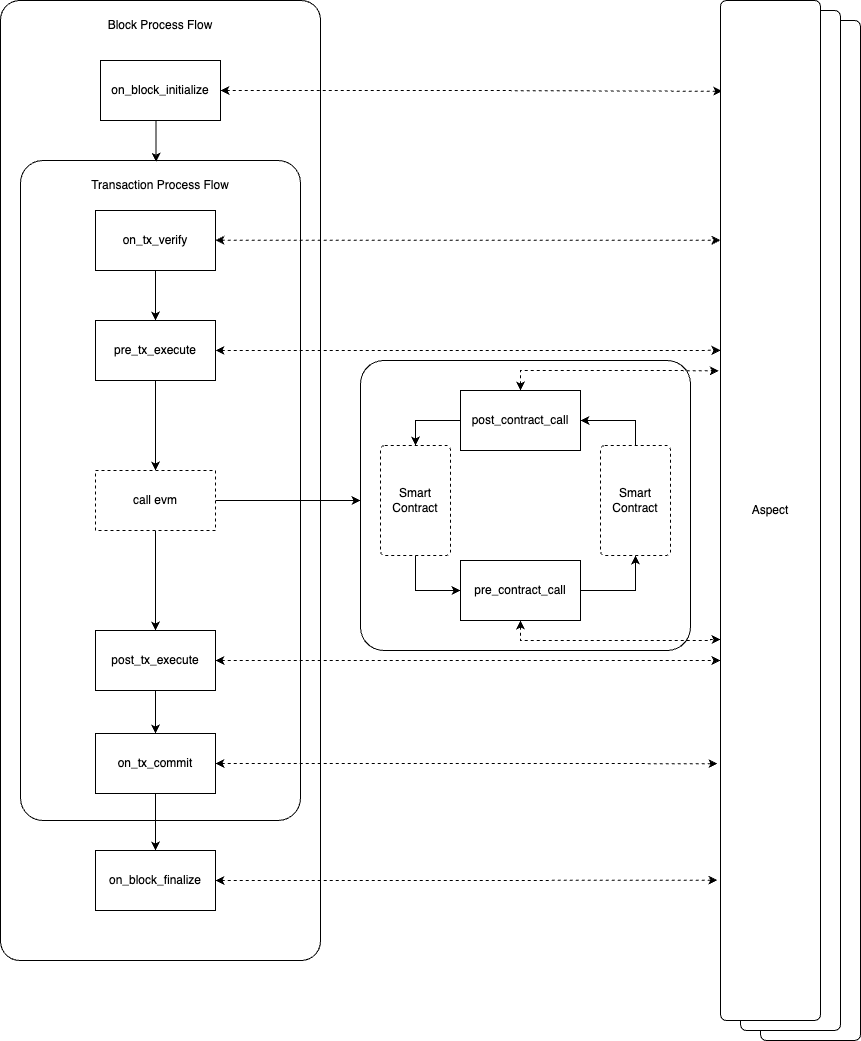
\includegraphics[width=0.4\linewidth]{sections/join-point-layout.png}
  \caption{Layout of join point.}
  \label{fig:join_point_layout}
\end{figure}

Figure \ref{fig:join_point_layout}  shows a list of join points that might be implemented. The following table \ref{tab:join-points-table} lists the description of the join points in which we describe what Aspect might do in those join points. 

\begin{longtable}{p{4cm}p{10cm}} % Adjust the column widths as desired
    \caption{Description of join points and their corresponding actions.}
    \label{tab:join-points-table} % Add a label for referencing
    \\
    \toprule
    \multicolumn{1}{c}{Join Point} & \multicolumn{1}{c}{Description} \\
    \midrule
    \endfirsthead
    
    \multicolumn{2}{c}{{\tablename\ \thetable{} -- continued from previous page}} \\
    \midrule
    \multicolumn{1}{c}{Join Point} & \multicolumn{1}{c}{Description} \\
    \midrule
    \endhead
    
    \midrule
    \multicolumn{2}{c}{{Continued on next page}} \\
    \endfoot
    
    \bottomrule
    \endlastfoot
    
    on\_block\_initialize & Activated prior to the preparation of the block proposal. Automated transaction is allowed to be inserted at this point. \\[20pt]
    on\_tx\_verify & Triggered following the transaction signature verification. The Aspect can introduce a customized transaction verification process, which takes precedence over the built-in process. \\[30pt]
    pre\_tx\_execute & Triggered prior to the transaction execution. At this stage, the account state remains pristine, allowing Aspect to preload information as necessary. \\[30pt]
    pre\_contract\_call & Triggered before the execution of the cross-contract call. At this stage, the state of the callee remains unaltered, providing the Aspect with an opportunity to preload any necessary information. \\[30pt]
    post\_contract\_call & Triggered after the cross-contract call is executed. The Aspect can then inspect the post-call state of the contract and make subsequent execution decisions. \\[30pt]
    post\_tx\_execute & Activated once the transaction has been executed and the account states have been finalized. Subsequently, Aspect can conduct a comprehensive review of the final execution state. \\[30pt]
    on\_tx\_committed & Triggered after the transaction has been finalized, and the modified states induced by the transaction have already been flushed into the state database. At this stage, Aspect can conduct post-processing activities, such as initiating an asynchronous task that can be executed in a future block. \\[60pt]
    on\_block\_finalize & Triggered after a block has been finalized. It permits the Aspect to submit an asynchronous task that can be executed in a future block. \\[30pt]
    % Add more rows if needed
\end{longtable}


Notably, the join point delivers an abstract definition, permitting implementation variations across different blockchains. This adaptability caters to differences in exposed join points, permissible operations at the join point, as well as other platform-specific considerations.

\subsubsection{Context}

The runtime context $C$ provides Aspects with information on transaction and block processing, including information such as modified states of smart contracts, emitted events, and raw data fields of the transaction. Formally: 

$$
C \equiv (c_b, c_t, c_a, c_e) \\ 
c \equiv (p_1, p_2,...) \\ p \equiv (p_{k}, p_{v})
$$

The context is structured as a collection of key-value pairs (formally, $p$), and when an Aspect requests a specific key (formally, $p_k$), the node will provide the most recent corresponding value (formally, $p_v$) at that point of processing. For instance, a $p_k$ `tx.origin.nonce` represents the nonce field’s value in the original transaction. Within the same $B$, It is essential that at a given $J$ for a specific $T$, all nodes in the blockchain network return the same $p_v$ for that $p_k$. This ensures the consistency of $c$, thereby aligning with the consensus mechanism. Each join point defines a specific group of $p$ that are accessible for an Aspect run on it.

\textbf{Context subsets.} All $p$ in the $C$ can be categorized into four subsets (formally, $c$). $c_{b}$ includes static information of $B$, such as block hash, validator(s) signature, etc. $c_{t}$ includes static information and real-time execution data of $T$, such as input data, transaction receipts, and state changes during execution. $c_a$ is a subset that allows modification by Aspects. Each Aspect has its own namespace in $c_a$, and Aspect can only modify $p$ in its own namespace while it’s limited that only able to read $p$ in other Aspect’s namespace. $c_e$ includes some environment variables of the node, such as the network id, etc.

\textbf{Context lifecycle.} The lifecycle of a context, $C$, is confined within a single block. When a block begins processing, a new context object is created for each transaction within that block. This context holds transaction-specific data and helps maintain state consistency throughout transaction execution. Once the block's processing completes — that is, all transactions within that block have been executed — the context is destroyed. It's important to note that this doesn't impact the blockchain's overall state or the results of the transaction, which are stored permanently on the blockchain. The context's purpose is merely to hold transient data that aids transaction execution and maintain state consistency within the scope of a single block.

\subsubsection{System Call}

In Aspect, a system call (formally, $\psi$) triggers the execution of a certain system module (formally, $M$). An $M$ can be stateful, it can maintain its own states (formally, $\varpi_{M}$). Formally: 

$$
\varpi_{M_{t+1}}=\psi(\varpi_{M_t},\psi_i)
$$

Each $\psi$ has a specific input (formally, $\psi_i$). If an $M$ is stateful, the corresponding $\psi$ will lead the state transition of the given $M$, $\varpi_{M}$. $M$ provides abilities to interact with the base layer’s functionality. For example, a specific $J$ after EVM execution can offer a system call that allows Aspect to create a “just-in-time” transaction. This transaction will be executed at the end of the block or right after the current transaction. System calls provide an essential interface between Aspect and the node.

\textbf{System Call Categories.} System calls, based on their distinct functionality, can be categorized into several groups: transaction management, block management, information maintenance, communication, and protection.

\begin{itemize}
  \item Transaction management system calls empower Aspects to construct and schedule just-in-time transactions.
  \item Block management system calls allow Aspects to participate in the block-proposing stage.
  \item Information maintenance system calls grant access to node-related data.
  \item Communication system calls enable interaction between Aspects, smart contracts, and native modules.
  \item Protection system calls allow Aspects to enforce transaction lifecycle rules.
\end{itemize}

Apart from these categories, unique system calls may be implemented in projects such as Artela or other blockchain platforms, aligning with their specific requirements.

$\psi$ is a blocking operation implying that the Aspect execution is paused and awaits the completion of $\psi$ before proceeding. If $\psi$ involves persistent state modification during execution, it is essential to ensure consistency between transaction states and the modifications made by $\psi$. This is crucial because a transaction may be reverted, which would discard its associated modifications. Furthermore, the design of $\psi$ should prioritize thread safety to effectively manage concurrent transaction executions.

\subsection{Aspect}

In this subsection, we provide a description of the Aspect's runtime, gas protocols, state storage procedures, validation processes, governance mechanisms, and upgrade methodologies.

Aspect is a dynamic and autonomous system-level extension for the blockchain. It is triggered in a specific join point, running securely within a sandboxed environment. Much like a smart contract, an Aspect can uphold its own state and proffers a programmable ownership interface, thereby facilitating a variety of governance approaches.

Aspect can also be conceptualized as an event-driven state machine, where an event might be the introduction of a new block or transaction at their different lifecycle stages. Commencing from the genesis state, the Aspect sequentially handles those events, culminating in its present state. The state transition ability provided by the Aspect can be formally defined as:

\[
\varpi_{t+1} \equiv \Gamma(\varpi_t,T)
\]
\[
\Gamma(\varpi,T) \equiv \iota(\varpi_{_{A}},\varpi_{_{S}},C,\sigma)
\]

Here, $\Gamma$ is the state transition function of Aspect which takes two inputs: current state $\varpi$ and transaction $T$. When an Aspect is triggered by a transaction $T$, state transition will be applied to the state $\varpi$. To expand $\Gamma$ in a more detailed function, it can be denoted as $\iota$ which takes four inputs: Aspect state $\varpi_a$, system module state $\varpi_s$, runtime context $C$, and world state $\sigma$.

\subsubsection{Structure}

The structure of an Aspect includes the following fields:

\begin{itemize}
  \item \textbf{Id ($A_i$):} Unique identifier of Aspect, 20-byte byte array.
  \item \textbf{Version ($A_{v}$):} This is a scalar value, equivalent to the number of version changes for the Aspect, starting from 1.
  \item \textbf{Type:} This refers to the kind of Aspect. Currently, the 'Built-in Aspect' is the only type defined in the white paper.
  \item \textbf{Byte Code ($A_{c}$):} This field refers to both current and historical versions of the Aspect code.
  \item \textbf{Governance Accounts ($A_{ga}$):} These accounts can implement governance actions concerning the Aspect. These actions include version upgrades, property changes, and version deprecation. Supported account types include EoA (Externally Owned Account), CA (Contract Account), and AA (Account Abstraction).
  \item \textbf{Settlement Accounts ($A_{sa}$):} The Aspect is not portrayed as an account on the blockchain, hence it cannot retain any assets. However, these settlement accounts are capable of holding assets and facilitating payments on behalf of Aspect. The base layer adheres to an authorization protocol, jointly established by Aspect and the settlement account, to ensure the security of the assets held in the settlement accounts.
  \item \textbf{Join Points ($A_{j}$):} This field represents all join points registered by the Aspect. It's a list of join point id $J_i$.
  \item \textbf{Bindings ($A_{b}$):} This field represents all binding relationships between the Aspect and various smart contracts. It's a list of binding relation records $b$.
  \item \textbf{Properties ($A_{p}$):} Properties represent immutable storage at Aspect runtime. It is read-only during the execution in join points. Properties are limited to undergoing modifications through the Aspect configuration process.
  \item \textbf{Storage ($A_s$):} Storage refers to mutable storage at Aspect runtime, which can be dynamically read from and written to during the execution in join points.
\end{itemize}

The state of Aspect ($\varpi_a$) can be defined with the following equivalence:

\[
\varpi_{_A} \equiv (A_{v},A_{c},A_{ga},A_{sa},A_{j}, A_{b},A_{p},A_{s})
\]

\subsubsection{Lifecycle}

An Aspect's lifecycle typically consists of deployment, upgrade, configuration, binding, execution, and destruction.

\textbf{Deployment.} This phase only occurs once. During deployment, it is necessary to specify the registered join points $A_{j}$, governance account $A_{ga}$, settlement account $A_{sa}$, and initial properties $A_{p}$. If the governance and settlement accounts are not specified, the signed EoA and caller contract account will be established as both. The deployment will initialize the state of Aspect as the following:

\[
\varpi_{_A} \equiv
\begin{cases}
    (1,A_c,A_{ga},A_{sa},A_{j},0,A_{p},0) & \text{if } A_{sa} > 0 \lor A_{ga} > 0 \\
    (1,A_c,S(T),S(T),A_{j},0,A_{p},0) & \text{otherwise}
\end{cases}
\]

Here, $A_{c}$ is the byte code of the Aspect; $A_{p}$ is the properties that will be initialized by the deployment; $S$ is the function of address recovery, which computes the sender address from the transaction signature. If the settlement account or governance account of Aspect is specified ($A_{sa} > 0 \lor A_{ga} > 0$), the settlement account and governance account of the Aspect will be set with the input, otherwise the sender of the transaction will be set as $A_{ga}$ and $A_{sa}$.

\textbf{Upgrade.} The upgrade process for an Aspect is flexible and can be initiated at any point after its deployment, with no limit to how many times it can occur. During the upgrade, both the byte code of the Aspect and its registered join points can be modified. The new code becomes effective starting from the next block after the upgrade transaction has been processed. The upgrade process is defined as the following:

\[
\varpi_{{t+1}_A} \equiv U(\varpi_t{_{_{A_c}}},\varpi_t{_{_{A_v}}},\varpi_t{_{_{A_j}}},A_c,A_j)
\]
\[
U(\varpi{_{_{A_c}}},\varpi{_{_{A_v}}},\varpi{_{_{A_j}}},A_c,A_j) \equiv ((\varpi_{_{A_c}} \oplus A_{c}),(\varpi_{_{A_v}} + 1),(\varpi{_{_{A_j}}} \oplus A_j)) 
\]

The upgrade process is captured by the upgrade function $U$ which takes the current code store of the Aspect ($\varpi{_{_{A_c}}}$), current Aspect version $\varpi{_{_{A_v}}}$ , join points of current Aspect ($\varpi{_{_{A_j}}}$), new Aspect byte code ($A_c$), and new Aspect join points ($A_j$) as inputs. The code store $\varpi{_{_{A_c}}}$ and join point store $\varpi{_{_{A_j}}}$ maintain all versions of Aspect code and corresponding join points. During the upgrade process, $A_c$ and $A_j$ will be added to $\varpi{_{_{A_c}}}$ and $\varpi{_{_{A_j}}}$ with $\varpi{_{_{A_v}}} + 1$ as their key. It's important to note that smart contracts can bind to the same Aspect across different versions. This is why both $\varpi{_{_{A_c}}}$ and $\varpi{_{_{A_j}}}$ are designed to support multi-version storage. In this way, the system ensures backward compatibility while still allowing for necessary upgrades and modifications.

We will discuss the specifics of upgrade authority within the governance section.

\textbf{Configuration.} The configuration can be activated at any time after deployment, and there is no limit to the number of times. The configuration process facilitates updates to the governance account $A_{ga}$, the settlement account $A_{sa}$, and various properties $A_p$. However, these configuration modifications will not come into play until the subsequent block. The state transition Aspect 

\[
\varpi_{_{A_{t+1}}} \equiv \Iota(\varpi_{_{A_t}}, A_{ga},A_{sa},A_p)
\]

Where $\Iota$ is the configuration process of Aspect which takes four inputs: current state of Aspect $\varpi_a$, new governance account $A_{ga}$, new settlement account $A_{sa}$, and updated properties $A_p$.

The particulars of configuration authority will be explained in the governance section.

\textbf{Binding.} The binding process can be activated at any time after deployment, and there is no limit to the number of times. The process allows the smart contract owner to bind the smart contracts to this Aspect. It is defined as a system procedure $f(b)$, which we will explain in detail in section 4.3.

\textbf{Execution.} Execution of Aspect can be triggered in different ways. We design two ways to trigger the Aspect:

\begin{itemize}
  \item \textbf{Triggered at join points:} This term refers to the activation of Aspects by join points. During a specific stage in its lifecycle, a transaction traversing a join point automatically triggers the Aspect associated with its callee. The execution can be defined as the following equivalence:
  \[
  (\varpi_{_{A_{t+1}}},\varpi_{_{S_{t+1}}},C_{t+1}) \equiv \iota(\varpi_{_{A_{t}}},\varpi_{_{S_{t}}},C_{t}, \sigma_t)
  \]
  Where $\iota$ is the state transition function of Aspect at a certain join point, which takes four inputs: state of Aspect ($\varpi_{a}$) and system modules $\varpi_{s}$, runtime context $C$, and world state $\sigma$. It makes the state transition and produces new $\varpi_{a}$, $\varpi_{s}$, and $C$.
  
  \item \textbf{Triggered by external calls:} Aspects can also embody external interfaces that may be invoked manually by an EoA (Externally Owned Account). These interfaces allow querying the Aspect or transitioning its state. The definition of the external call can be explained as $\iota'$:
  \[
  (\varpi_{_{A_{t+1}}},\varpi_{_{S_{t+1}}}) \equiv \iota'(\varpi_{_{A_{t}}},\varpi_{_{S_{t}}},\sigma_{t})
  \]
  Different from $\iota$, $\iota'$ cannot access runtime context $C$ because it isn't in a transaction or block process flow.
\end{itemize}

\textbf{Destruction.} A particular version of an Aspect can be destroyed if there are no associated smart contracts. Similarly, an Aspect can be destroyed if none of its versions are linked to any smart contract. The process of destroying an Aspect can be formally depicted as:
\[
D(A,\varpi_{_A}) \equiv \emptyset
\]
Where $D$ is the destruction process which takes an Aspect ($A$) and its state $\varpi_{_A}$ as inputs, and $D$ will erase the state data $\varpi_{_A}$ from the state storage, making it empty ($\emptyset$).

\subsubsection{Execution environment}

The execution of Aspect must meet the following requirements: determinism, isolation, efficiency, quantifiable computation cost, and flexible cost payment.

\textbf{Determinism.} The execution of Aspects will be performed by the entire network of validators. Operations that introduce indeterminism can undermine consensus. Therefore, features that may result in uncertain outcomes, such as multithreading, I/O operations, or dynamic typing, are not supported during execution.

The above characteristic can be formally defined as the following:
\[
\Xi_{A_{v_1}}(A, \varpi, C) \equiv \Xi_{A_{v_2}}(A, \varpi, C)
\]
Where $\Xi_{A}$ represents the execution environment of Aspect, it is a code execution function. If we input the same Aspect $A$, Aspect state $\varpi$, and runtime context $C$ into $\Xi_{A}$, each validator ($v_1$ and $v_2$) will achieve the same result.

\textbf{Isolation.} The execution of Aspects must be securely isolated to prevent the compromise of blockchain availability and security. Three levels of isolation are required for Aspect execution:

\begin{itemize}
  \item \textit{Isolation among Aspects:} Executions of individual Aspects must remain isolated. During the execution of one Aspect, no other Aspect should interfere with its current state. Protection against such interference must extend to both memory and storage.
  \item \textit{Isolation between Aspect and smart contract:} Aspect's execution does not infringe on the state integrity of a smart contract and vice-versa. The runtime should utilize a separate memory stack and storage state trie from the EVM. Direct access to each other's state or memory is disallowed, all the communications between Aspect runtime and the EVM should be done by message passing through the system call residing in the blockchain extension and base layers.
  \item \textit{Isolation between Aspect and base layer modules:} The blockchain base layer's memory stack and state storage should be obscured from Aspects to guard against intrusion into the base layer's execution processes. The only way for Aspect to communicate with the base layer is through the limited host APIs provided by the built-in runtime.
\end{itemize}

\textbf{Efficiency.} The execution of Aspects refers to additional processes that are added to the smart contract transaction execution. This implies that it introduces extra overhead to the transaction processing. The execution environment should achieve as near-native speeds as possible.

\textbf{Quantifiable computation cost.} The computational resources used by a transaction need to be limited to ensure that the total processing time stays within a reasonable range. This is particularly crucial for maintaining the efficiency and robustness of the blockchain network. In the case of Aspects, the total computational cost, or "gas cost", of a transaction is calculated as the sum of the individual gas costs of each operation performed by the Aspect and the smart contract. Formally:

\[
A_{c} \equiv (... \oplus W_{m} \oplus W_{n} \oplus ...  ) \oplus (... \oplus \psi_{m} \oplus \psi_{n} \oplus ...  )
\]
\[
g_{_A} \equiv (...+g_{_{W_{m}}}+g_{_{W_n}}+...) + (...+g_{_{\psi_m}}+g_{_{\psi_n}}+....)
\]

Each operation can be either a WebAssembly instruction (denoted as $W$) or a system call (denoted as $\psi$). The bytecode of an Aspect ($A_c$) consists of a series of these instructions and system calls. The total gas cost of the Aspect ($g_{_A}$) is the summation of the individual gas costs for each of these operations.

By quantifying and limiting these computational resources, we can ensure that the time required for consensus on the blockchain network is kept within acceptable boundaries. This is crucial for maintaining the network's speed and efficiency.

\textbf{Gas limit.} The Aspect system, like the smart contract execution system on the blockchain, has a gas limit mechanism to prevent infinite or resource-consuming executions. This limit ensures that an Aspect operation won't monopolize the system's computational resources or cause processing delays. Before the execution of an Aspect, a gas limit is set. This gas limit is then deducted throughout the execution of the Aspect for each operation or computational step. If an Aspect's execution attempts to exceed the assigned gas limit, the execution is halted, and any state changes made during that execution are reverted. This mechanism maintains the overall performance and stability of the blockchain system while allowing complex and resource-intensive operations to be performed in a controlled manner.

\textbf{Flexible cost payment.} The method for gas payment is adjustable for Aspect execution. The gas fee can be set to be charged from the caller, the settlement account, or both.



\subsubsection{Governance}

The governance procedures of Aspect are defined as system procedures. Operations such as Aspect deployment, upgrades, and configuration are managed by the Aspect system module. These governance procedures engage corresponding system module APIs to modify Aspect. Procedures can be expressed formally as the following:

\[
O \in (I, U, D) \\
V(\varpi_{ga},a) \equiv
\begin{cases}
1 & \text{if } \varpi_{ga} = a \\
0 & \text{otherwise}
\end{cases} \\
G(\varpi_{ga},T) \equiv V(\varpi_{ga},S(T)) \oplus O 
\]

The modification to an Aspect's State Transition Function (STF) can only be carried out by the governance account of that Aspect. Any operation ($O$) that could affect the STF of Aspect, whether it be a configuration ($I$), upgrade ($U$), or destroy ($D$) operation, must first pass a validation function ($V$). The validation function checks the given address ($a$) against the current governance account of the Aspect ($\varpi_{ga}$), allowing the operation to proceed only if they match. This ensures that only the authorized governance account can perform operations that modify the STF of an Aspect. This validation process forms part of the governance process ($G$), which takes both the governance account and the operation transaction ($T$) as inputs.

The governor of Aspect can be an Externally Owned Account (EoA), Account Abstraction (AA), or Contract Account (CA). Aspect owners are free to select the governance model that best suits their needs. For instance, should an Aspect require self-governance via utility tokens, it can be facilitated through AA.

\subsubsection{Settlement}

When the blockchain's base layer necessitates payment from the Aspect, the amount will be deducted from the settlement account tied to the Aspect. This settlement account is established through a bidirectional authentication process:

\begin{itemize}
  \item Aspect can set the settlement account in deployment or configuration operation.
  \item An authorization process will be initiated by the Aspect system module to verify that the settlement account has authorized this Aspect for settlement binding operation.
\end{itemize}

Once this bond is conclusively formed, the underlying protocol of the Aspect can execute debits without condition. Management of the Account funds' liquidity must be handled externally, as insufficient funds could result in a failed execution. The deductions the Aspect may incur include gas fees or service fees. We allow the Aspect to determine the payment methods flexibly with settlement account(s). Additionally, certain system calls may necessitate payable actions, which will also be deducted from this account by default.

\subsubsection{Programming features}

We design efficient, secure, and extension-style programming features for Aspect and support Aspect to act as an extended role in the blockchain. Those features include:

\begin{itemize}
  \item \textbf{Native Governance:} Aspect supports native governance, which means changes to Aspect's code, properties, and so on must be accomplished through system procedures defined by Aspect itself. During programming, crucial runtime parameters of the protocol can be placed in properties, such as those requiring governance like pausing the protocol or adjusting fees. Hence, value modifications can be directly completed by initiating governance via system procedures, eliminating the need for additional governance-related coding and external audits. Only the government accounts of the Aspect have the authority to operate these system procedures. Governance accounts can be extended into rich governance architecture through methods like CA, AA, etc. 
  \item \textbf{In-memory State:} To minimize the cost of state loading during execution, developers may opt to cache specific storage states in memory, particularly when the number of read operations significantly surpasses the number of write operations. To ensure that the use of an in-memory state meets the requirements of deterministic execution, as well as providing efficiency and lower costs than the state storage, its underlying implementation still encapsulates the state storage. The intermediate layer offers functionalities resembling those of memory.
  \item \textbf{Semantic-rich Transaction:} Aspect leverages runtime context to supplement the semantics of a transaction. For instance, a cryptographic Aspect authenticates the multi-party signature within a transaction prior to an EVM call and stores the verification result in the context. During transaction execution in EVM, the smart contract is able to reference this signature verification result, thus eliminating the need for independent verification. Thereby, by Aspect Programming, we are able to design a semantic-rich transaction. Both Aspects and smart contracts can utilize these semantics in runtime contexts to facilitate message exchanges.
  \item \textbf{Context Exchange:} In Aspect, communication occurs through the exchange of context. This communication can take place between different Aspects or between an Aspect and a smart contract. One such scenario might involve a previous Aspect writing the KYC (Know Your Customer) flag into a transaction, which a subsequent Aspect can then read to determine its own actions.
\end{itemize}

\subsubsection{Context layout}

Runtime context of Aspect refers to the information that Aspect can use and transmit during its execution. Runtime context is composed of two parts: join point contexts and Aspect context.

\textbf{Join point contexts.} Different join points have access to various contexts. These contexts include:

\begin{itemize}
  \item \textbf{Block Contexts:} This context, which is based on current blockchain data, is accessible at all join points. It allows for queries regarding block height, as well as calls to smart contracts, among other things.
  \item \textbf{Transaction Contexts:} This context refers to the current transaction state, and it is only available at transaction-related join points. The transaction context is composed of two major parts:
    \begin{itemize}
      \item The static part provides transaction-related data such as transaction hash, transaction sender, and so on.
      \item The information generated when processing the transaction such as signature verification result, smart contract call stack, and world state changes.
    \end{itemize}
\end{itemize}

\textbf{Aspect contexts.} Aspect context refers to an in-memory data object that can be shared among Aspects. Each Aspect has its own designated data area within the Aspect context isolated by the namespace, where only the owner Aspect has the write permissions, while others retain read-only access. Aspects can use this context to transmit messages based on a mutually agreed protocol. 

\textbf{Environment contexts.} Environment context contains the overall chain environment information, including chain id, current fork, and so on.

\subsubsection{Verification}

To ensure the integrity of Aspect execution across the network, an Aspect root will be recorded in each block. At the end of the block consensus, the validator will verify the correctness of the Aspect.

The transaction receipt ($R$) of Ethereum is composed of: the type of the transaction, $R_x$, the status code of the transaction, $R_z$, the cumulative gas used in the block containing the transaction receipt as of immediately after the transaction has happened, $R_u$, the set of logs created through the execution of the transaction, $R_l$ and the Bloom filter composed from information in those logs, $R_b$:

\[
R \equiv (R_x, R_z, R_u, R_b, R_l)
\]

Verification of the Aspect requires an additional field to be added into the transaction receipt data structure, we denoted it as $R_c$, which represents the context hash of Aspect:

\[
R_c \equiv keccak(keccak(keccak(C_{a_0}),C_{a_1})...)
\]
\[
R \equiv (R_x, R_z, R_u, R_b, R_l, R_c)
\]

\textbf{Result Validation.} Each Aspect context is preserved within an in-memory lexicographically ordered map. The context root, which represents the hash of the entire Aspect context content, is calculated with the key-value pairs in the context map and documented within the transaction receipt. This procedure facilitates a concise verification of the integrity and authenticity of the Aspect contexts. Validators can confirm the Aspect result by re-executing the Aspect and comparing the resultant hash with the $R_c$ recorded in the transaction receipt.

\subsection{Binding}

Binding is the process that establishes a connection between an Aspect and a smart contract. If a smart contract binds with an Aspect, the transaction call to the smart contract will trigger the execution of the Aspect.

\[
(...,A_m, A_n,...) \equiv \Eta(a_{sc}, \forall b)
\]
\[
b \equiv (a_{sc},A_i, A_v, A_p)
\]
\[
f_{b}(b)
\]

Here, $H$ stands for a process that loads all bound Aspects of the given smart contract account address; $b$ represents the binding relation record of Aspect and smart contract, it is composed of four major pieces of information: smart contract address ($a$), bound Aspect id ($A_i$), bound Aspect version ($A_v$), and execution priority ($A_p$); binding relationships can be established via a system procedure $f_{b}$.

\subsubsection{Binding Process}

Aspect binding can be initiated through an EoA transaction or a smart contract call. To prevent unauthorized bindings for both smart contracts and Aspects, the binding process necessitates a dual-way authorization between the Aspect and the smart contract. This is crucial as the state of each can be impacted when they are combined. If this dual-way authorization is successful, the binding relationship will be recorded. Consequently, when the smart contract is triggered either by an EoA transaction or a smart contract call, the associated Aspect will also be invoked for execution.

A binding transaction or call includes the following information:

\begin{itemize}
  \item \textbf{aspect id:} This is the ID of the Aspect to bind.
  \item \textbf{aspect version:} This represents the version of the Aspect to bind. Please note, a smart contract can only bind to one version of an Aspect at a time.
  \item \textbf{contract address:} This is the address of the smart contract which will bind the Aspect.
  \item \textbf{priority:} This determines the execution order of the Aspect when triggered by the smart contract call. Aspects bound to a smart contract will be executed in a sequence. dApp developers can orchestrate this execution order according to their specific requirements.
\end{itemize}

The binding process $f(b)$ can be defined as:

\[
f(b) \equiv X(A_i) \oplus F(A_i, A_v,a_{sc},b_p)
\]

Where $F$ is the binding process. $F$ persists the binding relationship into the Aspect state $\varpi_a$ of $A_i$ and it takes four inputs: id of the Aspect ($A_i$), version of the Aspect ($A_v$), smart contract address ($a_{sc}$), and execution priority ($b_p$).

$X$ is the authorization function implemented in the smart contract. It mandates that the binding Aspect must be authorized by the smart contract $a_{sc}$. The authorization function can be formally defined as:

\[
X(A_i) \equiv
\begin{cases}
  1 & \text{if id of A is authorized} \\
  0 & \text{otherwise}
\end{cases}
\]

The function $X$ receives the id of the Aspect ($A_i$) as an input and performs a validation check. If $A_i$ is authorized, the function will return 1, indicating that the binding operation is valid and can proceed. If $A_i$ is not authorized, the function will return 0, indicating that the binding operation is invalid and should be aborted. This authorization process $X$ adds flexibility because it allows smart contracts to define their own unique validation processes. This can be particularly beneficial in systems where different smart contracts may have different requirements and standards for what constitutes an authorized operation.
